
\documentclass[journal]{IEEEtran}

\usepackage{graphicx}
\usepackage{hyperref}

\ifCLASSINFOpdf
\else
\fi

% *** SUBFIGURE PACKAGES ***

% figure.

\hyphenation{op-tical net-works semi-conduc-tor}


\begin{document}
\title{ControlShield: Network Security \\and Forensics for \\Industrial Control Systems}

\author{Juan~Ortiz,~(MSEE),
        Rushi~Sharma,~(MSEE),
        David~Jessup,~(BSECE),
        and~Harrison~Hsu~(BSECE)
\thanks{The authors are students from California Polytechnic Pomona.}}




\markboth{ECE 4311.01 --- Network Forensics, Fall 2026 Final Project}%
{ControlShield: Network Security and Forensics for Industrial Control Systems}

\maketitle

% in the abstract or keywords.
\begin{abstract}
Industrial Control Systems (ICS) are critical components of modern automated
infrastructure, encompassing sectors such as logistics, manufacturing, energy
and utilities. Security and forensics on Programmable Logic Controllers (PLC)
are paramount due to the potential consequences of cyber threats and
vulnerabilities. This project presents ControlShield, an Industrial PLC Guardian
that provides integrated intrusion detection and prevention capabilities to
safeguard ICS environments.

\\ \hspace*{1em}The experiments conduct greybox analysis on a simulated ICS
network with a TM212CE24T PLC, HMIS5T HMI and a managed TP-Link TL-SG105E switch.
The PLC Guardian is a Windows based python application that monitors the network
for malicious activity and provides real-time alerts and mitigation actions. The
design theory is a fully integrated PLC IPS that communcates directly with the
PLC to prevent malicious activity.

\\ \hspace*{1em}The results demonstrated the effectiveness of ControlShield in
near real-time detection using port mirroring and packet analysis. The PLC
Guardian successfully identified and mitigated various attack scenarios, including
exploitation of exposed services such as diagnostics web portal and Modbus TCP attacks.
There is also experiments conducted to blackbox footprinting and reconnaissance
attacks for system discovery.

\\ \hspace*{1em}In conclusion, ControlShield provides a comprehensive solution for
enhancing the security and resilience of Industrial Control Systems.
\end{abstract}

\begin{IEEEkeywords}
Industrial control systems, programmable logic controllers, network security,
intrusion detection and prevention, network forensics, cybersecurity.
\end{IEEEkeywords}

\IEEEpeerreviewmaketitle

\section{Introduction}

\IEEEPARstart{T}{he} goal of this report is to document the experiments conducted for
the ControlShield project. For a bit of context, automated control systems has been
ever evolving since the late 1960s (see Figure~\ref{fig:relay-ladder}).

\begin{figure}[t]
  \centering
  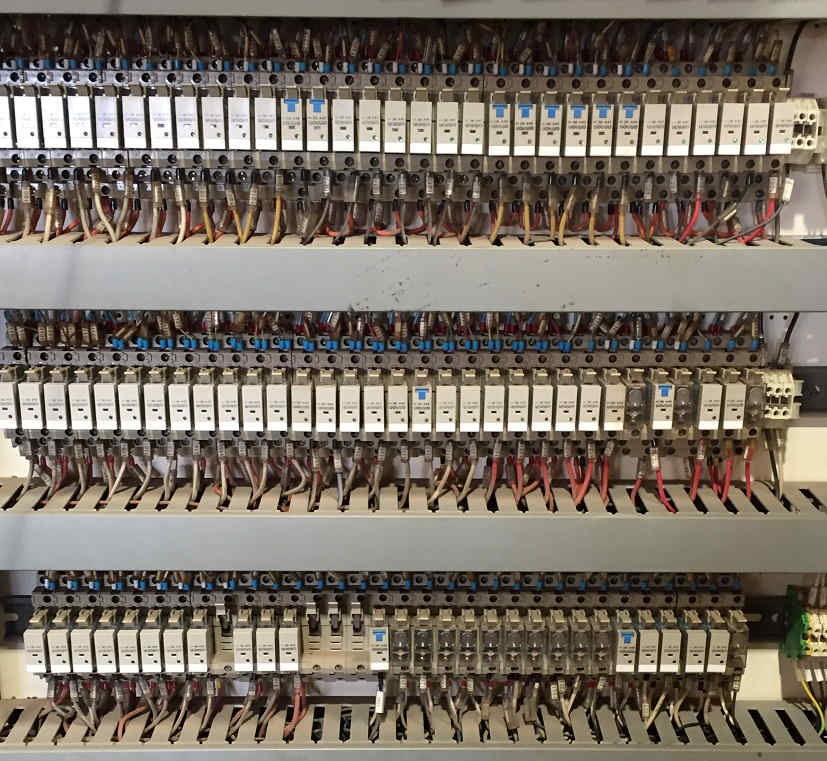
\includegraphics[width=\columnwidth]{images/RelayLadder.jpg}
  \caption{A hard wired control system using traditional rack
  implementations of timers, relays, contactors, etc.}
  \label{fig:relay-ladder}
\end{figure}

\\Automation using relay logic is labor intensive, difficult to troubleshoot
and hard to modify. Making it nearly immutable to system integrations or future
upgrade implementations. The PLC (see Figure~\ref{fig:retro-plc}) sought to replace
these hard-wired relay systems and revolutionize manufacturing and facility
automations.

\begin{figure}[t]
  \centering
  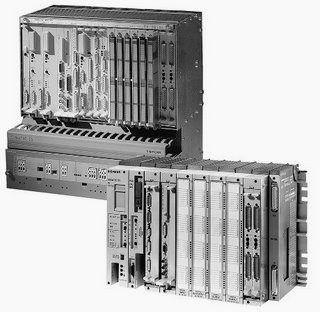
\includegraphics[width=\columnwidth]{images/Modicon084.jpg}
  \caption{The Modicon 084 was early development of the Programmable
    Logic Controller designed in 1968 by Dick Morley's Bedford Associates.}
  \label{fig:retro-plc}
\end{figure}

\\Since their inception the PLC has taken dominance in the automation and
industrial controls sectore. With the evolution of technology these controllers
have adapted numerous features including web servers, network communication,
safety mechanisms and standardized protocols to name a few. With the modernization
of this technology, the threat landscape has also followed suit. The programmable
logic controller has several layers of abstraction on top of conventional
x86 and ARM based controllers. Malicious Cyber Actors (MCA) and foreign entities
familiar with these architectures can find Common Vulnerabilities and
Exposures (CVE) to carry out attacks.

\\Earlier this year the FBI reported MCA's causing operational disruption to
nine water systems in Michigan. The target being multiple mature end-of-life (EOL)
Rockwell Allen-Bradley controllers namely the MicroLogix 1100 and 1400 series
(see~\cite{fbi-ics-2026}). The conduit for this attack was open-network facing
controllers. These device were placed in a manner where the internal control
network was bridged to public services. MCA's used this bridge to remote into
all of the PLCs and change crucial device configurations such as setting
passwords and changing IP addresses. This very simplistic vulnerability caused
loss of water pressure and flooding. Even reportedly could've allowed untreated
ground water to seep in to piping system. ControlShield is a cyber attack
simulation project to integrate Network Intrusion Prevention (NIPS) and
Detection Systems (NIDS) into a control network.

\section{Scenario}
A water facilitation plant has been compromised by an MCA.
This person manages to gain direct access to an internal control network similarly
to the threat in Michigan. This entity does not have any previous knowledge of
the automation infrastructure but does have the technicality to apply off-the-shelf
tooling like NMAP, Wireshark and Python. This project will prove even without
the expertise of a professional, critical damage can still arrise from basic
computering skills in the hands of a malicious actor. 

\\Some other potential threats can stem from insiders, specifically personnel
who have complete access and knowledge of the internal system. The PLC software used
in this simulation generates useful documentation that is reminiscent of
proprietary documentation in real world applications (see Figure~\ref{fig:pdf}).
Insider threats have access to this documentation, though in this simulation
the attacker won't have this knowledge, fingerprinting the system can give
just as good detail.

\begin{figure}[t]
  \centering
  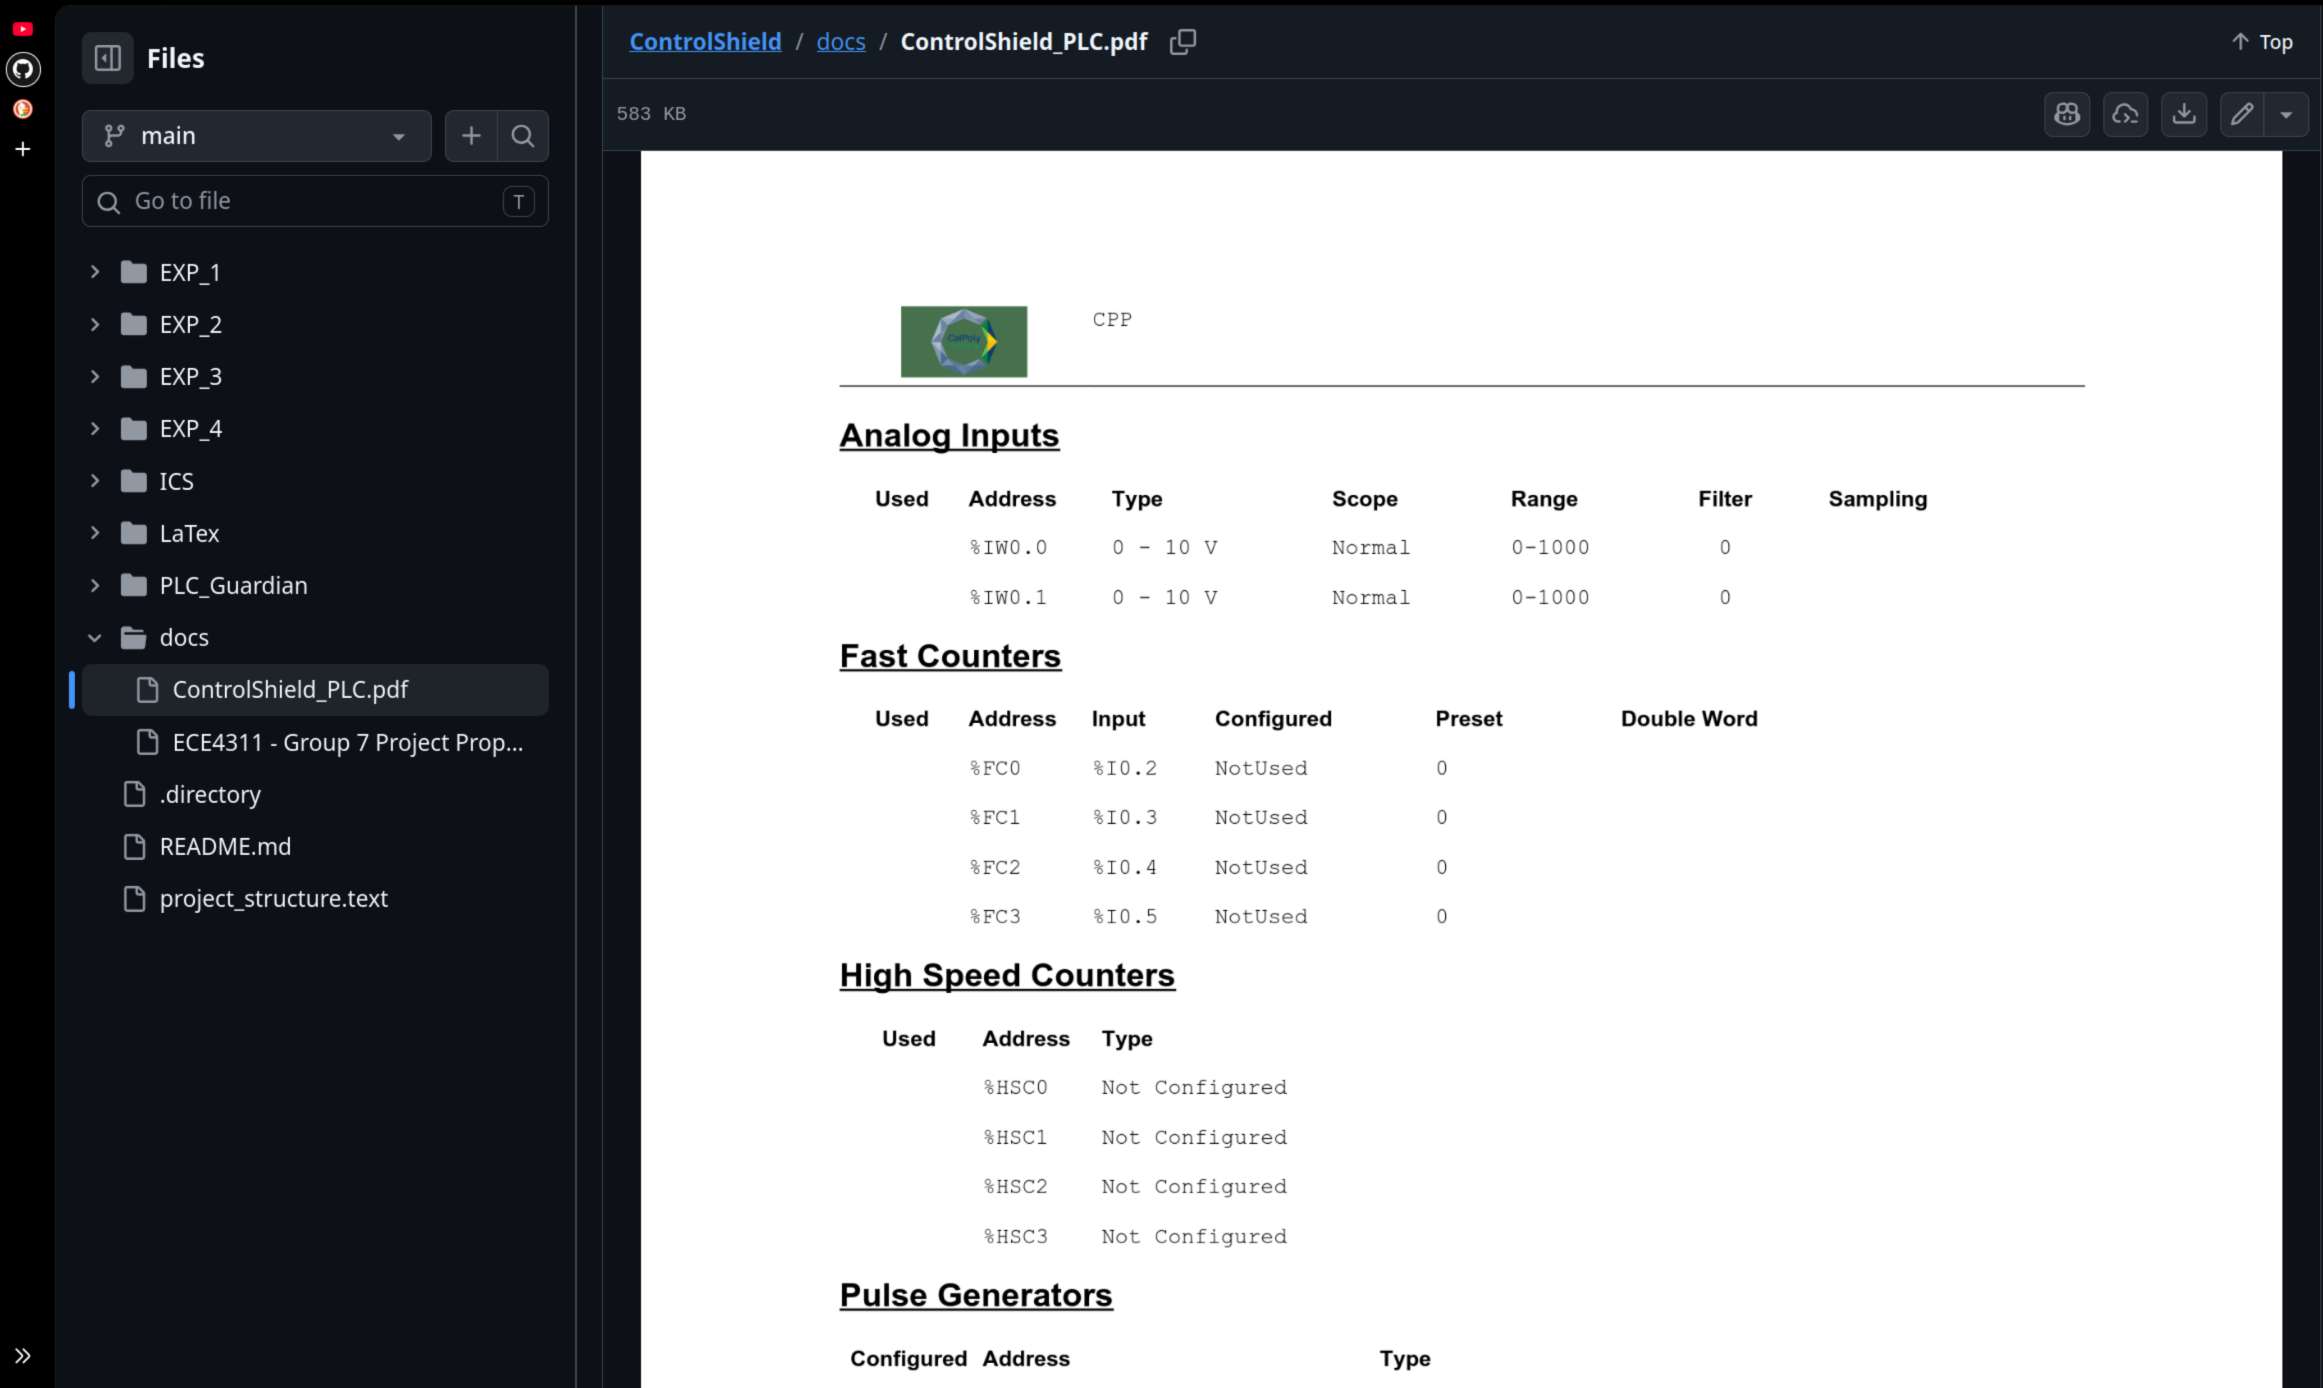
\includegraphics[width=\columnwidth]{images/pdfdoc.png}
  \caption{This documentation directly outlines the automation logic and
    device configuration for the simulated control system.}
  \label{fig:pdf}
\end{figure}

\section{Methodology}
This simulation will be conducted on physical real-world hardware in an isolated
test environment. The environment network layout can be visualized in the diagram
provided (see in Figure~\ref{fig:topology}). This configuration will mimick a basic
managed switch network where all traffic is port mirroed to the PLC Guardian. From
here the Guardian will monitor the traffic with a custom application created to
detect and prevent intrusions within the network.

\\In order to properly intercept malicious packets before they reach a device, an
inline set up will need to be configured. The thought process for going with a port
mirrored configuration is that most existing facilities have 24 hour operations,
meaning there is very little downtime to re-configure an entire network. Also the
criticality and risk assessment in implementing an entirely different network structure
could result in unintended communication issues. By simply copying the entire
traffic of the network and sending it directly to the newly installed Guardian.

\begin{figure}[t]
  \centering
  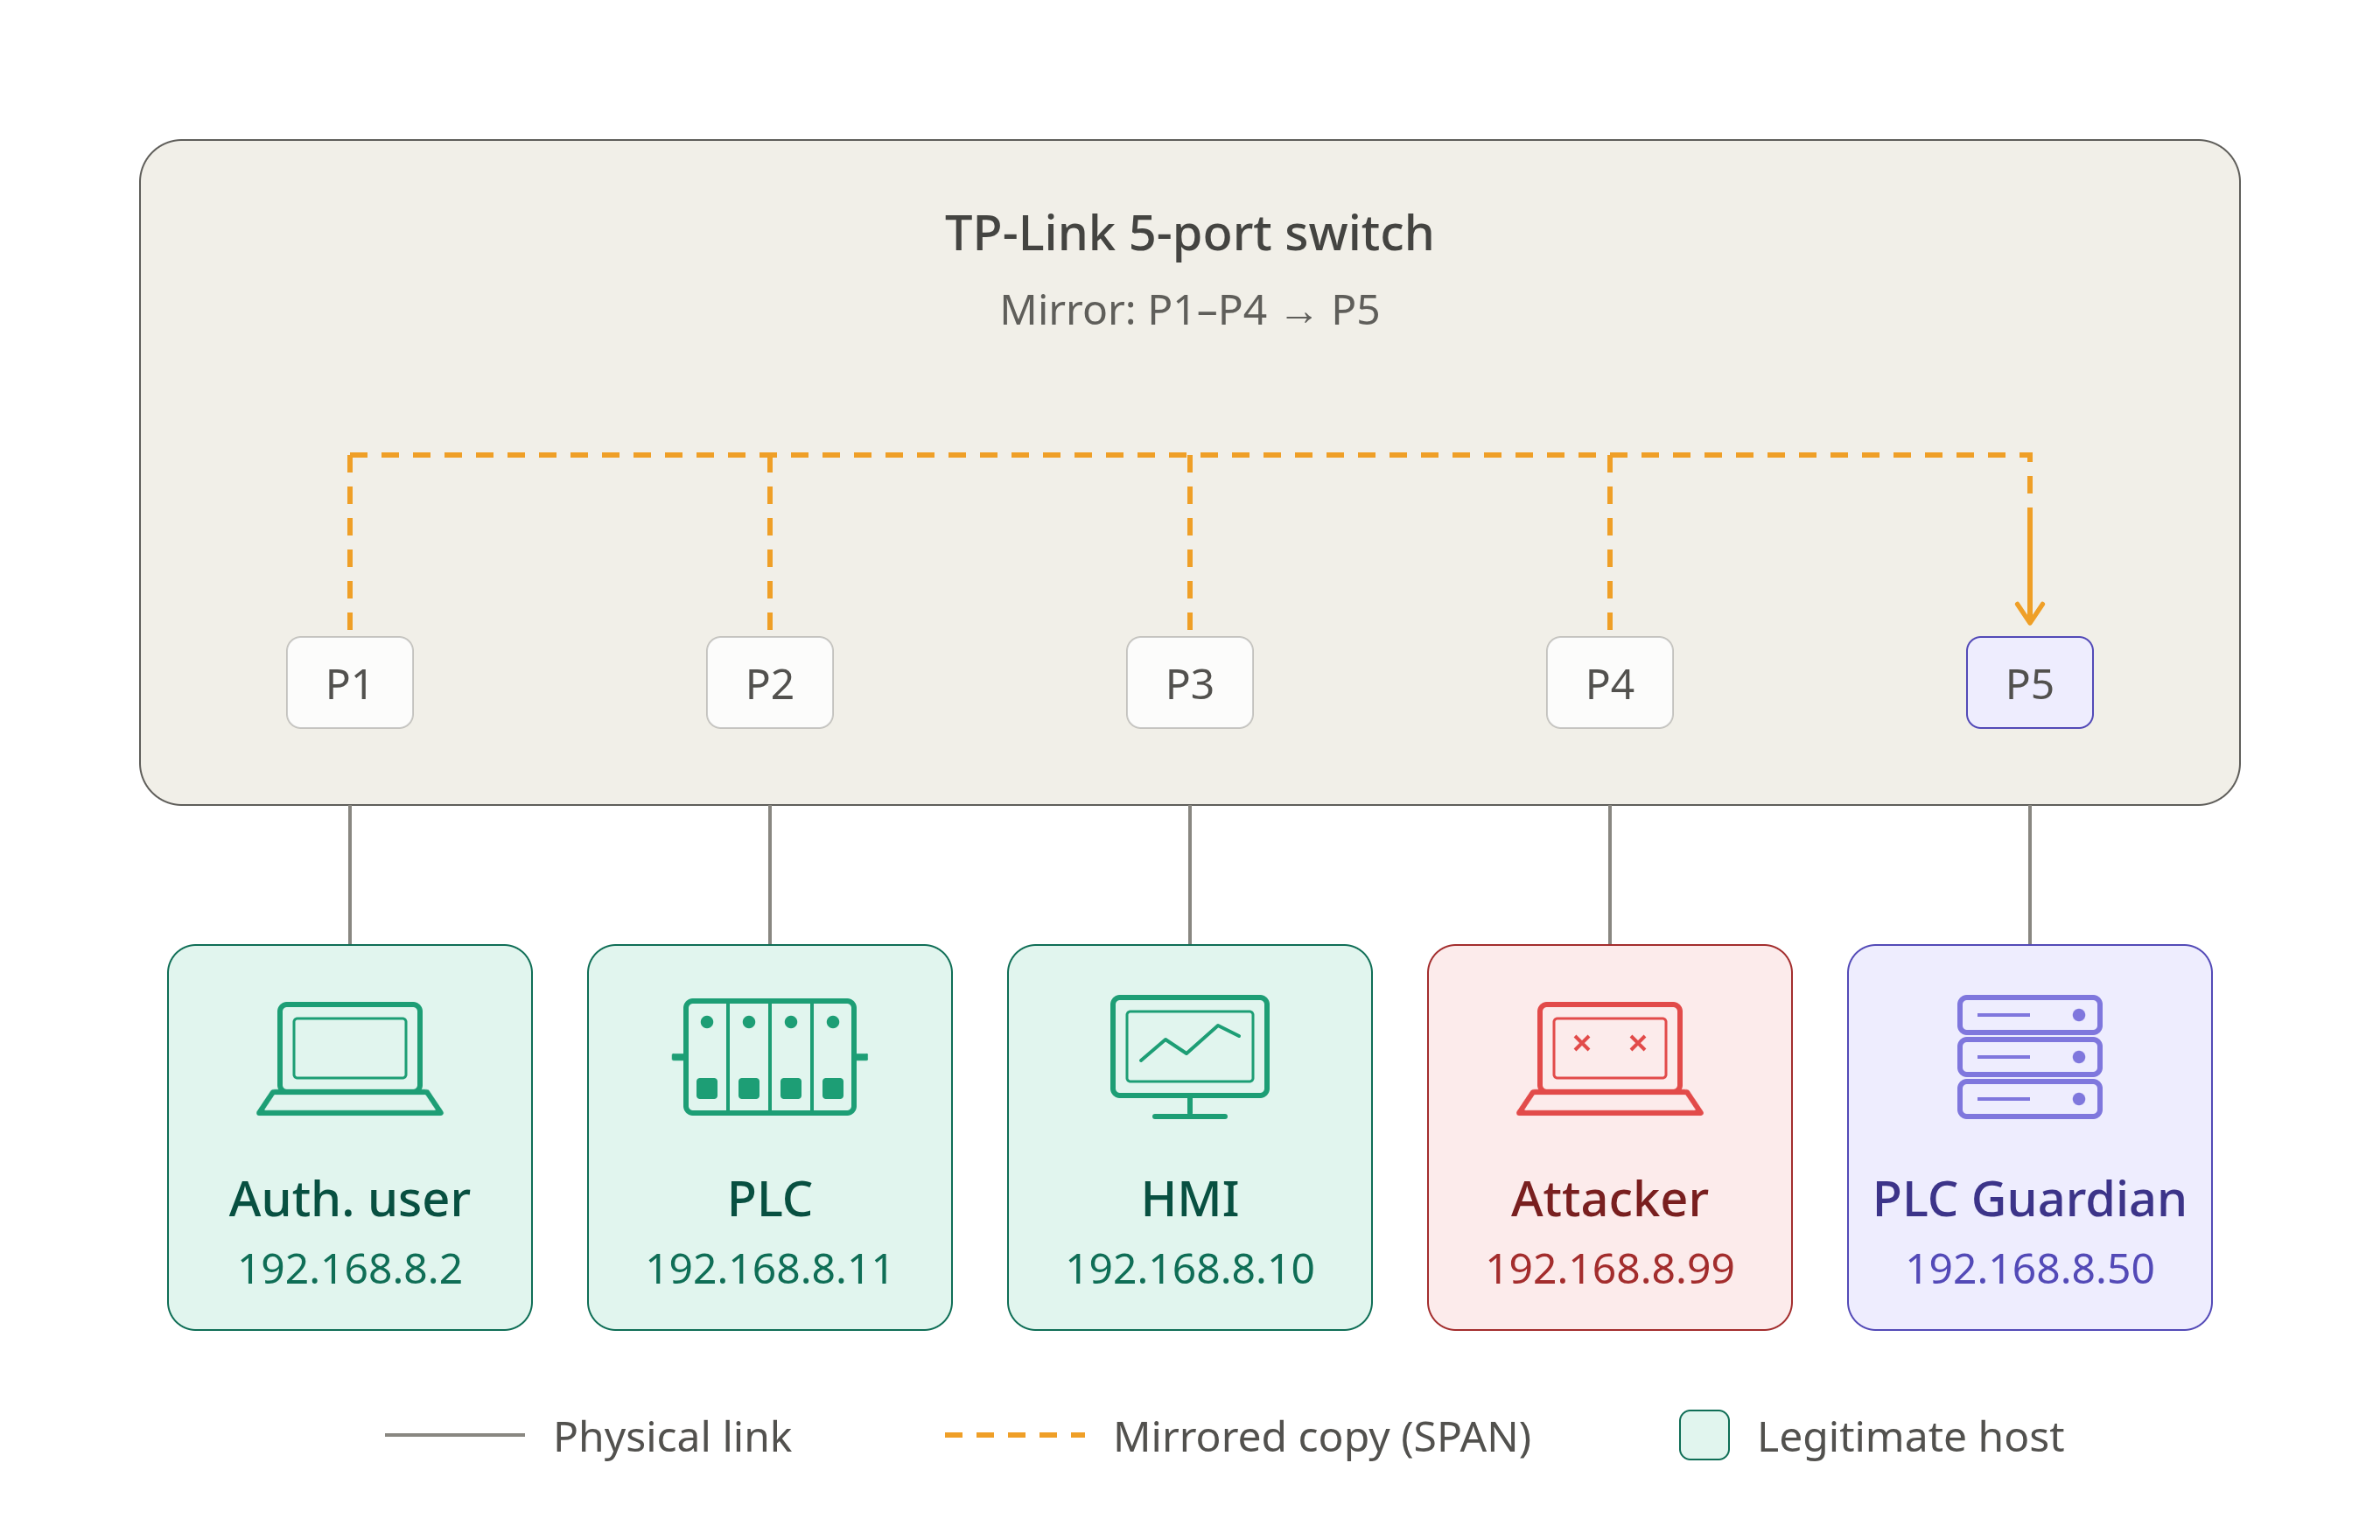
\includegraphics[width=\columnwidth]{images/topology.png}
  \caption{Simulated Network topology for the ControlShield project.}
  \label{fig:topology}
\end{figure}

\\The hardware consists of a TM212CE24T Schneider Electric PLC, this is a an industrial
that is used in automating smaller applications such as a conveyors, water pumps,
PID control loops and many other real world applications. This controller is
significantly more capable than the MicroLogix in the Michigan Wasterwater facility.
Next is the Human Machine Interface (HMI) model HMIS5T also by Schneider Electric. This is a
graphical user interface for operating the system in the field. A custom user
interface was developed to simulate a water tank filling up until hitting a set
threshold. 
 
 

\subsection{System Design}
Subsection text here.

\subsubsection{ICS Network Architecture}
Subsubsection text here.

\subsubsection{PLC Guardian Design}
Subsubsection text here.

\subsection{Experiments and Results}
Subsection text here.


\subsubsection{Baseline Network Traffic Analysis}
Subsubsection text here.

\subsubsection{Exposed Services Exploitation}
Subsubsection text here.

\subsubsection{Modbus TCP Attack}
Subsubsection text here.

\subsubsection{Intrusion Prevention and Mitigation}
Subsubsection text here.

\section{Conclusion}
The conclusion goes here.





% if have a single appendix:

% use appendices with more than one appendix
% then use \section to start each appendix
% starts a section numbered zero.)


\appendices
\section{Proof of the First Zonklar Equation}
Appendix one text goes here.

\section{}
Appendix two text goes here.


% use section* for acknowledgment
% \section*{Acknowledgment}


The authors would like to thank...


\ifCLASSOPTIONcaptionsoff
  \newpage
\fi




% references section

\begin{thebibliography}{2}

\bibitem{fbi-ics-2026}
Federal Bureau of Investigation, ``Malicious Cyber Actors Targeting Water and Wastewater Sector Internet-Facing Programmable Logic Controllers,`` 2026.
[Online]. Available: \href{https://www.fbi.gov/investigate/cyber/alerts/2026/malicious-cyber-actors-targeting-water-and-wastewater-sector-internet--facing-programmable-logic-controllers-causing-operational-disruptions}{FBI Cyber Alert}}

\bibitem{controlshield-repo}
J. Ortiz et al., ``ControlShield,'' GitHub repository. [Online]. Available:
\href{https://github.com/juanrortiz/ControlShield}{ControlShield GitHub repository}.

\end{thebibliography}

% biography section

\begin{IEEEbiographynophoto}{John Doe}
Biography text here.
\end{IEEEbiographynophoto}


\begin{IEEEbiographynophoto}{Jane Doe}
Biography text here.
\end{IEEEbiographynophoto}






\end{document}
